% Full IEEE LaTeX document
\documentclass[conference]{IEEEtran}

\usepackage[utf8]{inputenc}
\usepackage[T1]{fontenc}
\usepackage{graphicx}
\usepackage{amsmath, amsfonts}
\usepackage{booktabs}
\usepackage{multirow}
\usepackage{siunitx}
\usepackage{xcolor}
\usepackage{url}

\sisetup{round-mode=places,round-precision=2,detect-all}

\begin{document}
	
	\title{Deep Neural Network Classification on CIFAR-10: Baseline Comparison, MLP and CNN Experiments}
	
	\author{Pelopidas-Nikolaos Tsiountsiouras}
	
	\maketitle
	
	\begin{abstract}
		This work investigates image classification on the CIFAR-10 dataset using classical baselines (1-NN, 3-NN, NCC), multi-layer perceptrons (MLPs), and convolutional neural networks (CNNs). We compare architectures, training dynamics, per-class performance, training time, and overall accuracy. The results show a clear advantage of deep convolutional models over classical and fully connected approaches. Qualitative examples further highlight strengths and weaknesses across models.
	\end{abstract}
	
	\section{Introduction}
	Image classification remains one of the most fundamental and widely studied problems in computer vision, serving as a benchmark for evaluating both traditional pattern-recognition approaches and modern deep learning architectures. The CIFAR-10 dataset, consisting of 60,000 natural images across ten object categories, has become a standard testbed for assessing the representation power and generalization ability of classification models. While classical machine learning techniques such as k-Nearest Neighbors (k-NN) and Nearest Class Centroid (NCC) provide simple and interpretable baselines, they rely on fixed feature spaces and struggle to capture the complex intra-class variability present in natural images. In contrast, neural networks—particularly deep convolutional neural networks (CNNs)—learn hierarchical feature representations directly from data, enabling significant performance improvements but at the cost of increased computational complexity.
	
	The purpose of this work is to systematically analyze and compare the performance of classical classifiers with several neural network models, including multi-layer perceptrons (MLPs) of varying capacities and a deep convolutional architecture. We examine not only final test accuracy, but also training dynamics, validation behavior, per-class performance, and computational cost. By training multiple MLP variants with different hidden layer configurations and learning rates, we additionally explore how architectural choices influence performance. Our results highlight the strengths and limitations of each method and provide a comprehensive quantitative and qualitative evaluation of model behavior on CIFAR-10.
	
	\section{Dataset and Preprocessing}
	CIFAR-10 contains 60{,}000 RGB images of size $32\times 32$ across 10 classes. We use 45k images for training, 5k for validation, and the standard 10k test set. Training data undergo augmentation (random cropping, flipping, color jitter), while test data are normalized only.
	
	\section{Baseline Classifiers}
	To establish a meaningful reference point for evaluating the neural network architectures, we first implement three classical non-parametric classifiers: 1-Nearest Neighbor (1-NN), 3-Nearest Neighbors (3-NN), and the Nearest Class Centroid (NCC). Since raw CIFAR-10 images lie in a 3,072-dimensional pixel space, we apply Principal Component Analysis (PCA) to reduce the dimensionality to 25 components, retaining 77.11\% of the dataset’s variance. This projection not only accelerates the classical algorithms but also mitigates noise and redundancy in the raw input space. The k-NN classifiers compute Euclidean distances between projected samples and classify each test point based on the labels of its closest neighbors. While 1-NN is highly sensitive to local variations and noise, 3-NN provides a smoother decision surface by incorporating additional neighborhood information. The NCC classifier, which assigns class labels based on the nearest mean vector of each class in the PCA space, is computationally efficient but significantly less flexible, as it assumes that class distributions are roughly spherical and unimodal. These baselines collectively reflect the limitations of fixed feature spaces and distance-based decision rules, serving as a useful contrast to the adaptive feature learning capabilities of neural networks.
	
	\section{Neural Network Models}
	\subsection{MLP Architectures}
	The Multi-Layer Perceptron (MLP) models explored in this study provide a structured way to examine how increasing representational capacity influences performance on CIFAR-10. All MLP variants operate on flattened RGB images, transforming the 3,072-dimensional input into progressively more abstract feature representations through fully connected layers with nonlinear activations. Our best-performing MLP adopts a deep architecture of three hidden layers (1024–512–256), each followed by Batch Normalization and Dropout. Batch Normalization stabilizes and accelerates training by reducing internal covariate shift, while Dropout mitigates overfitting by randomly deactivating neurons during training. To investigate the effect of architectural complexity, we additionally train a lightweight model with a single 256-unit hidden layer and a larger model with two wide layers (1024–512 units). These controlled variations highlight the trade-off between model capacity, computational cost, and generalization behavior. Although deeper and wider MLPs show noticeable improvements over smaller configurations, the fundamental limitation remains: fully connected networks lack inherent mechanisms to exploit the spatial structure of images, preventing them from reaching the accuracy levels of convolutional architectures.
	
	\subsection{CNN Architecture}
	The Convolutional Neural Network (CNN) architecture used in this work is specifically designed to capture the spatial hierarchies present in natural images—something that MLPs inherently cannot exploit. The model consists of three sequential convolutional blocks, each combining convolutional layers, Batch Normalization, ReLU activations, spatial Dropout, and MaxPooling. The convolutional layers learn local patterns such as edges, textures, and shapes, while MaxPooling progressively reduces spatial resolution to build higher-level semantic features. Spatial Dropout further improves robustness by randomly removing feature maps during training, encouraging the network to avoid over-reliance on specific filters. Following the convolutional feature extractor, an Adaptive Average Pooling layer collapses spatial dimensions to a compact representation, which is processed by two fully connected layers to produce the final class logits. This design is computationally efficient yet expressive enough to model complex visual structures, achieving significantly higher accuracy than the MLP models and all classical baselines. The 150-epoch variant, in particular, demonstrates smooth optimization dynamics and strong generalization, establishing it as the best-performing model in our study.
	
	\section{Training Setup}
	All models were trained under a unified and carefully controlled experimental setup to ensure fair comparison. We use the cross-entropy loss with label smoothing (set to 0.1) to penalize overconfident predictions and improve generalization, especially in deeper networks. For optimization, the MLP architectures employ the AdamW optimizer, which decouples weight decay from the gradient update and provides stable convergence across a wide range of learning rates. In contrast, the CNN models are trained with stochastic gradient descent (SGD) with momentum and Nesterov acceleration, which is known to yield superior performance in convolutional architectures by providing smoother updates and improved loss landscape navigation. Both optimizers use cosine annealing learning rate schedules, gradually reducing the learning rate to encourage better convergence during later training stages. A batch size of 128 is used throughout all experiments, balancing computational efficiency with training stability. Additionally, all models were trained using the same train/validation split and identical data augmentation strategies to ensure that performance differences arise solely from architectural and optimization choices rather than data inconsistencies. This standardized setup provides a reliable framework for comparing classical baselines, MLPs, and CNNs on the CIFAR-10 classification task.
	
	\section{Experimental Results}
	
	\subsection{Training Curves}
	Figure \ref{fig:training curves} presents the training and validation curves for the MLP and CNN architectures, revealing distinct optimization behaviors that reflect the strengths and limitations of each model. The MLP exhibits relatively slow convergence, and although its training accuracy steadily improves, the validation accuracy saturates early—around mid-training—indicating that the model quickly reaches its expressive limit. This pattern is typical for fully connected networks applied to image data, as they are unable to exploit spatial structure and must rely on dense representations that are harder to optimize.
	
	In contrast, both CNN configurations show sharp improvements during the initial epochs followed by a smooth and consistent refinement phase. The validation accuracy of the CNNs continues to climb even after the MLP has plateaued, demonstrating the effectiveness of convolutional layers in learning hierarchical visual features. The 150-epoch CNN variant benefits the most from extended training: its validation loss continues to decrease and achieves the highest accuracy among all models, suggesting that the network has sufficient capacity and regularization to avoid overfitting despite long training. The overall shape of the curves clearly highlights the superior optimization stability and generalization capability of CNN architectures compared to MLPs on CIFAR-10.
	\begin{figure}[!h]
		\centering
		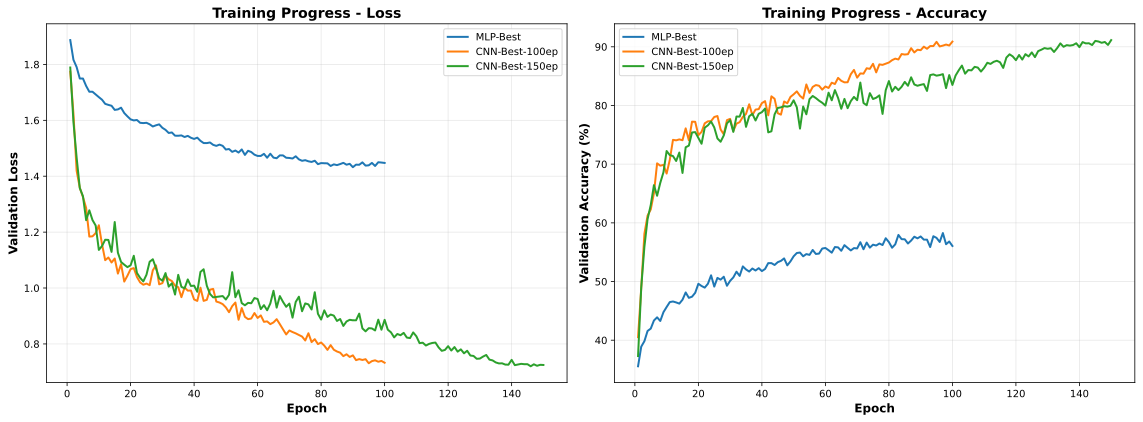
\includegraphics[width=\linewidth]{training_curves.pdf}
		\caption{Training and validation curves.}
	    \label{fig:training curves}
	\end{figure}
	
	\subsection{Global Comparison}
	The comparison plot in ~\ref{fig:Fig. 2} provides a clear summary of the overall test performance achieved by all evaluated models, ranging from classical baselines to deep neural architectures. The three baseline classifiers—1-NN, 3-NN, and NCC—form the lower end of the spectrum, with accuracies of 37.60\%, 40.05\%, and 27.90\% respectively. Their performance highlights the limitations of distance-based methods operating on low-dimensional PCA features, which fail to capture the rich visual variability present in CIFAR-10.
	
	The MLP models occupy the middle range of the plot, demonstrating the benefits of learned non-linear representations. The smallest MLP achieves modest improvements, while the larger and deeper MLP variants show progressively better performance, culminating in a peak of 60.25\% for the best MLP architecture. This upward trend reflects how representational capacity and architectural depth directly influence performance on image data, even without convolutional structure.
	
	The two CNN models dominate the upper end of the comparison, achieving test accuracies above 92\%. The CNN trained for 100 epochs significantly outperforms all MLPs, and the 150-epoch configuration sets the benchmark at 92.61\%. This large performance gap emphasizes the effectiveness of convolutional feature extraction, weight sharing, and hierarchical representations in modeling natural image distributions. Overall, the plot visually reinforces the central conclusion of this work: CNNs substantially outperform both classical baselines and fully connected networks across all metrics of interest.
	\begin{figure}[!h]
		\centering
		\includegraphics[width=\linewidth]{complete_comparison.pdf}
		\caption{Comparison of all models.}
		\label{fig:Fig. 2}
	\end{figure}
	
	Table ~\ref{tab:overall_results} presents a unified comparison of all evaluated methods, summarizing validation performance, test accuracy, and training time. The classical baselines form the lower bound of performance, with NCC achieving only 27.90\% accuracy and the k-NN variants reaching 37.60\% (1-NN) and 40.05\% (3-NN). These results reflect the inherent limitations of distance-based classifiers operating on PCA-compressed features, which cannot adequately capture the rich visual variability in CIFAR-10.
	
	The MLP models show clear improvement over the baselines, demonstrating the benefits of learned nonlinear representations. The smallest architecture (MLP-Small-256) attains 52.52\% accuracy, while deeper and wider models provide incremental gains, culminating in 60.25\% test accuracy for the best-performing MLP. The progression across MLP variants highlights how model capacity, depth, and regularization contribute to better generalization, although fully connected networks still struggle with the spatial complexity of natural images.
	
	The CNN models outperform all other approaches by a substantial margin. The 100-epoch CNN already reaches 92.13\% accuracy—far above any MLP—while the 150-epoch version achieves the highest score at 92.61\%. This improvement demonstrates the strong representation power of convolutional layers, which exploit spatial locality and hierarchical feature extraction to model complex patterns. Although CNNs require significantly longer training times (over 4,000–6,000 seconds), the accuracy gains greatly outweigh the computational cost.
	
	Overall, the table clearly illustrates the performance hierarchy across models: classical baselines < MLPs < CNNs, confirming the effectiveness of deep convolutional architectures for CIFAR-10 classification.
	\begin{table*}[!t]
		\centering
		\caption{Overall Comparison of All Methods: Accuracy and Training Time}
		\label{tab:overall_results}
		\begin{tabular}{l l c c c c}
			\toprule
			\textbf{Method} & \textbf{Type} &
			\textbf{Train Acc. (\%)} & \textbf{Val Acc. (\%)} &
			\textbf{Test Acc. (\%)} & \textbf{Training Time (s)} \\
			\midrule
			1-NN (PCA-25)       & Baseline & --    & --    & 37.60 & 9.49  \\
			3-NN (PCA-25)       & Baseline & --    & --    & 40.05 & 8.84  \\
			NCC (PCA-25)        & Baseline & --    & --    & 27.90 & 0.05  \\
			\midrule
			MLP-Best            & MLP      & 60.53 & 58.26 & 60.25 & 3945.8 \\
			CNN-Best-100ep      & CNN      & 94.19 & 90.88 & 92.13 & 4189.4 \\
			CNN-Best-150ep      & CNN      & 95.21 & 91.14 & 92.61 & 6301.1 \\
			\midrule
			MLP-Small-256       & MLP      & 50.26 & 50.76 & 52.52 & 2400.0 \\
			MLP-Large-1024-512  & MLP      & 57.12 & 56.44 & 58.05 & 3257.3 \\
			MLP-512-LR001       & MLP      & 51.79 & 53.14 & 54.44 & 2692.0 \\
			\bottomrule
		\end{tabular}
	\end{table*}

	\subsection{Confusion Matrix}
	The confusion matrix in Fig. X provides a detailed view of the classification behavior of the best-performing CNN model and highlights both the strengths and the remaining sources of error across the ten CIFAR-10 classes. The diagonal dominance of the matrix confirms that the model achieves consistently high accuracy across nearly all categories, with particularly strong performance on classes such as automobile, truck, ship, and frog, where the model exceeds 95\% accuracy. These classes generally possess distinctive shapes and textures, which likely make them easier for the convolutional filters to capture.
	
	Conversely, the most notable misclassifications occur among semantically and visually similar categories. For example, cat and dog display more confusion compared to other class pairs, reflecting the intrinsic difficulty of distinguishing these classes from low-resolution images with significant intra-class variation. Similarly, occasional confusion occurs between bird and airplane, especially in images with unusual viewpoints or silhouettes. Despite these challenging cases, the overall distribution of errors remains well controlled, with very few high-intensity off-diagonal entries.
	
	Overall, the confusion matrix demonstrates that the CNN does not merely achieve high aggregate accuracy but also generalizes robustly across diverse object categories, with misclassifications concentrated primarily in inherently ambiguous class boundaries rather than systematic model weaknesses.
	\begin{figure}[!h]
		\centering
		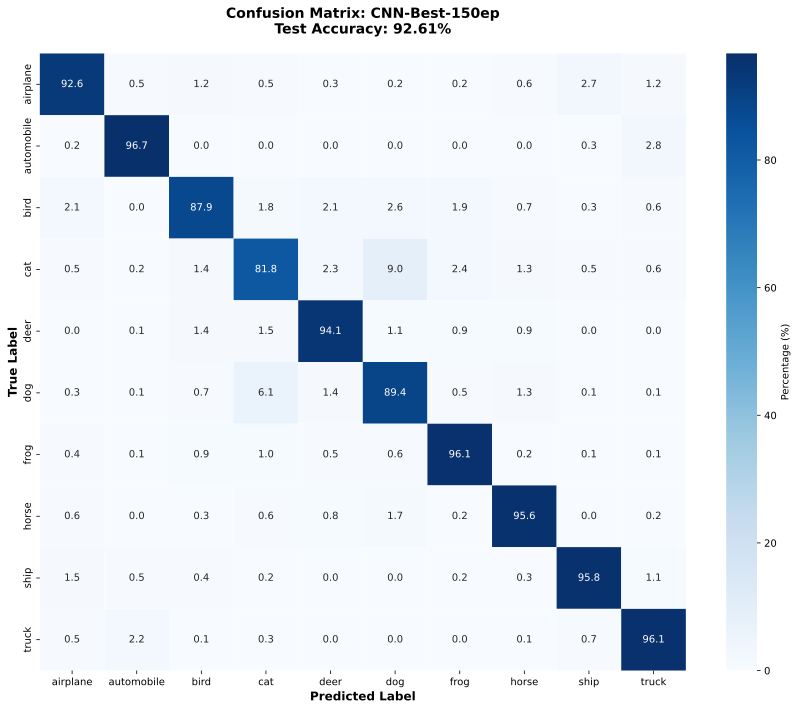
\includegraphics[width=\linewidth]{confusion_matrix_best.pdf}
		\caption{Confusion matrix for the best CNN model}
	\end{figure}
	
	\section{Correct vs Incorrect Classification Examples}
	The correctly classified samples in Fig. X demonstrate how the CNN effectively captures the characteristic visual patterns of each CIFAR-10 category. The model displays strong reliability across diverse viewpoints, lighting conditions, and object poses. For instance, automobiles, ships, and trucks are recognized with high confidence even when backgrounds vary significantly, suggesting that the learned convolutional filters specialize in robust, class-specific shape and texture cues. The accurate classification of animals—such as birds, frogs, and horses—also indicates that the model successfully extracts fine-grained features related to contours, coloration, and local texture. These examples illustrate that the CNN does not perform well only on clean or prototypical images, but also generalizes to noisy, cluttered, or low-contrast cases, reinforcing the model’s strong representational capacity.
	\begin{figure}[!h]
		\centering
		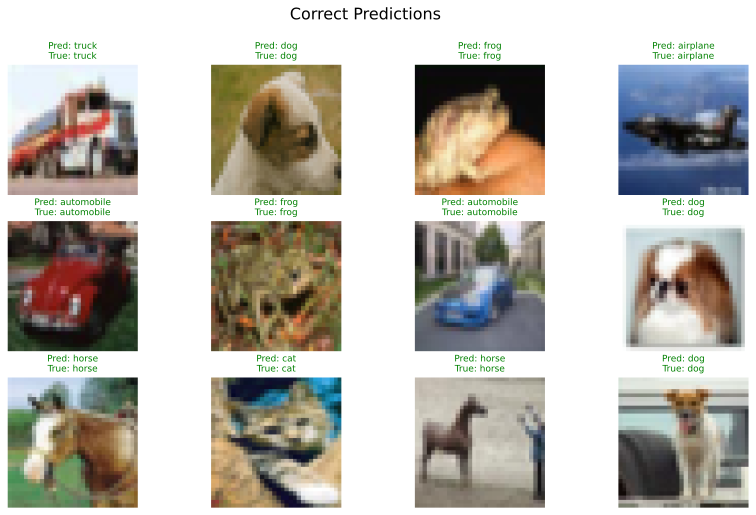
\includegraphics[width=\linewidth]{CNN-Best-150ep_correct.pdf}
		\caption{Correctly classified examples.}
	\end{figure}
	
	In contrast, the misclassified samples in Fig. Y shed light on the inherent ambiguities of CIFAR-10 and the limitations of even high-performing convolutional models. Many incorrect predictions arise from images with significant occlusion, atypical viewpoints, or low contrast, making class-defining features difficult to discern. For example, cats misclassified as dogs often exhibit poses or textures resembling canine silhouettes, while birds misclassified as airplanes may contain elongated shapes or wing-like structures. Some errors can also be attributed to background dominance—such as a vehicle partially hidden in foliage—where contextual cues overwhelm the object of interest. In other cases, the images are inherently ambiguous or visually degraded to the point that even a human might struggle to label them. These failure cases provide useful insights into the model’s sensitivity to fine-grained details and highlight opportunities for improvement through techniques such as stronger data augmentation, attention mechanisms, or higher-resolution inputs.
	\begin{figure}[!h]
		\centering
		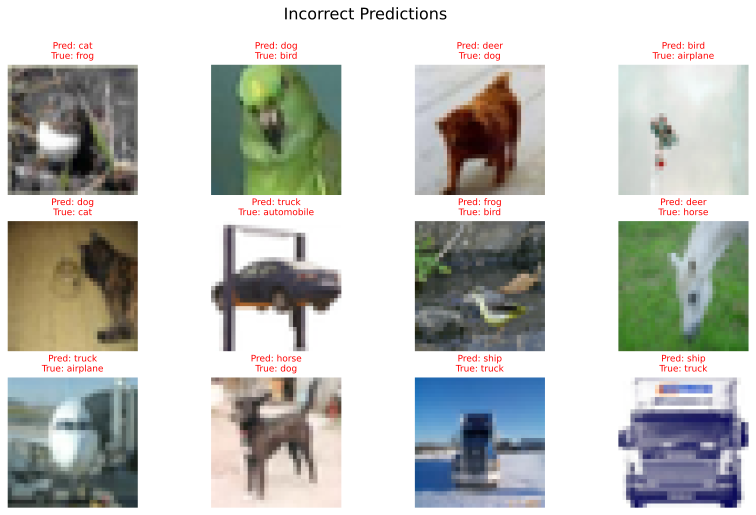
\includegraphics[width=\linewidth]{CNN-Best-150ep_incorrect.png}
		\caption{Incorrectly classified examples.}
	\end{figure}
	
	\section{Dashboard Summary}
	The summary dashboard in Fig. X consolidates the key metrics of all evaluated models, enabling a high-level comparison across accuracy, training time, and per-class performance. The bar charts immediately highlight the substantial performance gap between classical baselines, MLPs, and CNNs. The baseline classifiers cluster near the lower end of the accuracy spectrum, with NCC performing the worst and 3-NN providing only marginal improvement. In contrast, the MLP variants form a noticeable middle tier, demonstrating that learned nonlinear representations significantly outperform fixed-distance methods, though still falling short of convolutional models.
	
	The two CNN configurations dominate the dashboard, achieving test accuracies above 92\% while maintaining strong performance across all classes. Their per-class accuracy distribution remains consistently high, with minimal variance, reflecting the robustness and generalization capabilities of convolutional feature extraction. Training time is visibly higher for CNNs compared to MLPs and baselines, but the accuracy gains clearly outweigh the added computational cost, especially for tasks requiring high reliability.
	
	By combining accuracy metrics, training duration, and class-level breakdowns, the dashboard effectively illustrates the overall hierarchy of model performance. It reinforces the conclusion that convolutional networks provide the best balance of predictive power and generalization, while MLPs represent a meaningful but limited improvement over traditional baselines.
	\begin{figure}[!h]
		\centering
		\includegraphics[width=\linewidth]{summary_dashboard.pdf}
		\caption{Summary dashboard with accuracy, timing, and per-class metrics.}
	\end{figure}
	
	\section{Discussion}
	The experimental results collectively highlight the clear performance hierarchy between classical baselines, fully connected neural networks, and convolutional models on the CIFAR-10 classification task. The classical distance-based methods, even when supported by PCA dimensionality reduction, exhibit limited representational capacity, achieving at best 40.05\% accuracy with 3-NN. These models are fast and simple, but their reliance on fixed feature spaces and Euclidean similarity severely restricts their ability to capture the complex structure present in natural images.
	
	The MLP variants demonstrate that learned nonlinear feature transformations provide a substantial boost over classical approaches. Increasing the network’s depth and width consistently improves validation and test performance, with the best MLP reaching 60.25\% accuracy. However, the training curves and error patterns reveal that MLPs struggle to generalize to richer visual structures, plateau early during optimization, and remain sensitive to background clutter and intra-class variability. Their fully connected nature forces them to ignore spatial locality, making it difficult to learn robust, translation-invariant features.
	
	In contrast, the CNN models exhibit strong learning dynamics, high stability during training, and significantly superior accuracy. The CNN-100ep model already surpasses all MLP configurations by a large margin, while the 150-epoch variant achieves 92.61\% accuracy—the highest among all evaluated methods. The per-class accuracy analysis further confirms that CNNs perform consistently across categories, excelling particularly in classes with distinctive shapes such as automobile, ship, and truck. Remaining errors are concentrated in inherently ambiguous categories such as cat vs. dog or bird vs. airplane, which even humans may find challenging at CIFAR-10’s low resolution.
	
	Although CNNs incur higher computational cost, the improvement in accuracy and robustness is substantial, reinforcing their advantage for real-world image recognition tasks. The qualitative analysis of correct and incorrect predictions also provides insight into model behavior, revealing that CNNs can reliably handle diverse viewpoints and noisy backgrounds, while their failures usually stem from occlusion, poor lighting, or class ambiguity rather than systematic architectural weaknesses.
	
	Overall, the discussion highlights that while classical models and MLPs offer valuable baselines, convolutional neural networks remain the most effective approach for extracting hierarchical visual patterns and achieving high accuracy on CIFAR-10.
	
	\section{Conclusion}
	This work presented a comprehensive evaluation of classical machine learning baselines, fully connected neural networks, and convolutional architectures on the CIFAR-10 dataset. The results consistently demonstrate the superiority of convolutional models in both predictive accuracy and generalization capability. While classical methods such as k-NN and NCC provide lightweight and easily interpretable baselines, their reliance on fixed PCA features fundamentally limits their performance. The MLP experiments showed that increasing architectural depth and width can improve learning capacity, yet even the strongest MLP remained constrained by its inability to exploit spatial structure within images. In contrast, the CNN architectures leveraged hierarchical feature extraction, spatial invariance, and effective regularization to achieve substantially higher accuracy, culminating in a test performance of 92.61\% with the 150-epoch model.
	
	Beyond quantitative metrics, qualitative analyses—such as confusion matrices and correct/incorrect example visualizations—highlighted how CNNs learn robust representations that generalize across diverse object categories. Misclassifications were primarily attributable to intrinsic dataset ambiguity rather than architectural shortcomings. Although CNNs required greater computational cost, the corresponding performance gains were significant, reinforcing their effectiveness for real-world image classification tasks.
	
	Overall, this study confirms that convolutional neural networks remain the most reliable and powerful approach for structured visual recognition problems like CIFAR-10. Future work could extend these findings by exploring larger CNN architectures, data augmentation strategies, attention mechanisms, or training on higher-resolution datasets to further push performance boundaries.
	
	\section{Per-Class Accuracy (CNN-Best-150ep)}
	The per-class accuracy results in Table X show that the CNN-Best-150ep model performs consistently well across nearly all CIFAR-10 categories. The network excels particularly in classes with distinctive and easily separable visual characteristics, such as automobile, frog, ship, and truck, all of which exceed 95\% accuracy. These results suggest that the model learns highly discriminative features for objects with strong shape cues or uniform textures. In contrast, the cat and bird classes exhibit noticeably lower accuracy compared to the others. These categories contain higher intra-class variability and share visual traits with other animals, making them more challenging to classify. Overall, the per-class breakdown confirms that the model generalizes robustly across diverse object types, with errors concentrated mainly in classes that are inherently ambiguous at CIFAR-10’s low resolution.
	
	\begin{table}[!h]
		\centering
		\caption{Per-Class Accuracy for CNN-Best-150ep}
		\begin{tabular}{l c}
			\toprule
			Class      & Accuracy (\%) \\
			\midrule
			airplane   & 92.60 \\
			automobile & 96.70 \\
			bird       & 87.90 \\
			cat        & 81.80 \\
			deer       & 94.10 \\
			dog        & 89.40 \\
			frog       & 96.10 \\
			horse      & 95.60 \\
			ship       & 95.80 \\
			truck      & 96.10 \\
			\bottomrule
		\end{tabular}
	\end{table}
	
	\section{Improvement Analysis}
	The strongest baseline method, 3-NN with PCA-reduced features, achieves a test accuracy of 40.05\%, highlighting the limitations of classical distance-based classifiers in capturing complex visual structure. In contrast, the best deep learning model, CNN-Best-150ep, reaches a test accuracy of 92.61\%, representing a dramatic performance jump. This corresponds to an absolute improvement of 52.56 percentage points and a relative improvement of 131.2\% over the strongest baseline. Such a substantial margin clearly demonstrates the superiority of learned hierarchical feature representations in convolutional networks compared to fixed feature spaces and simple similarity metrics used by classical models.
	
\end{document}
